\documentclass[aspectratio=169, xcolor=dvipsnames]{beamer}
\hypersetup{pdfpagemode=FullScreen}
\beamertemplatenavigationsymbolsempty
\setbeamertemplate{caption}{\raggedright\insertcaption\par}
\usepackage[utf8]{inputenc}
\usepackage[spanish]{babel}
\usepackage{siunitx}
\usepackage{graphicx}
\usepackage{xcolor}
\usepackage{amsmath}
\usepackage{esint}
\usepackage{biblatex}
\usepackage{multicol}
\usepackage{listings}

\definecolor{myblue}{rgb}{0.29, 0.5, 0.94}

\title{Aplicaciones de Sistemas Embebidos con Doble Núcleo}
\subtitle{Introducción a FreeRTOS}
\author[Fabrizio Carlassara - Laboratorio de Sistemas Embebidos]{
\includegraphics[scale=0.15]{resources/images/utn_logo.png}}
\institute{UTN FRA\\Departamento de Ingeniería Electrónica\\Laboratorio de Sistemas Embebidos}
\date[]{\today} 
\usetheme{Warsaw}
\usecolortheme[named=myblue]{structure}
\setbeamertemplate{headline}{}

\begin{document}

\frame{\titlepage}
\begin{frame}{Introducción a FreeRTOS}{Índice}
\begin{multicols}{2}
\tableofcontents
\end{multicols}
\end{frame}

\section{FreeRTOS}
\begin{frame}{Introducción a FreeRTOS}{Por qué FreeRTOS?}
\begin{columns}
\begin{column}{0.5\textwidth}
\begin{itemize}
    \item Tareas y pseudo paralelismo de ejecución.
    \item Gestión fina de tiempo.
    \item Prioridades de eventos y tareas.
    \item Lógica más modular.
    \item Manejo dinámico de recursos.
    \item Porteado a múltiples platformas.
\end{itemize}
\end{column}
\begin{column}{0.5\textwidth}
\begin{figure}
\centering

\includegraphics[width=0.75\linewidth]{resources/images/freertos_logo.png}
\end{figure}
\end{column}
\end{columns}
\end{frame}

\section{Memoria}
\subsection{Segmentos de memoria}
\begin{frame}{Introducción a FreeRTOS}{Segmentos de memoria}
\begin{columns}
\begin{column}{0.4\textwidth}
\begin{figure}
\centering
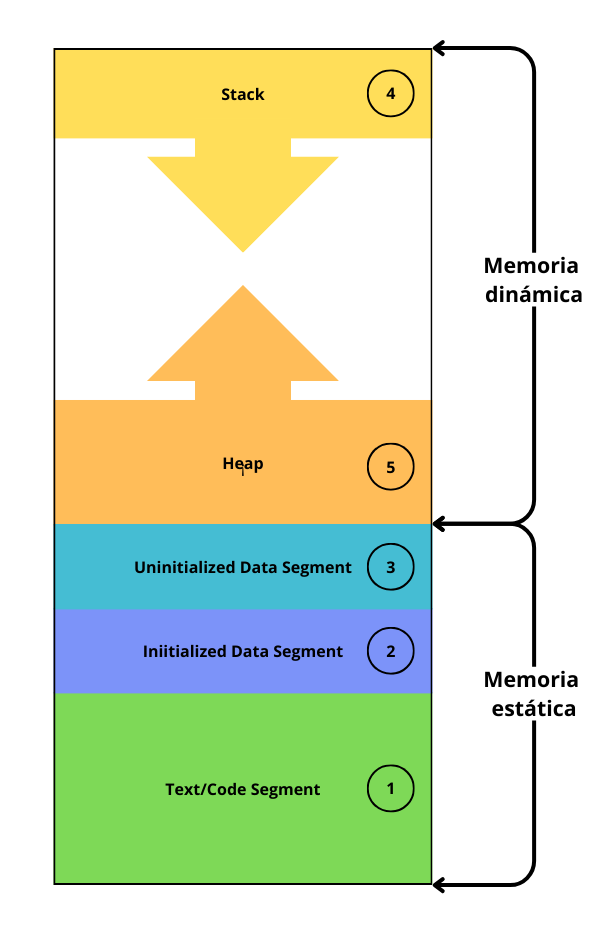
\includegraphics[width=0.7\linewidth]{resources/images/memory_layout.png}
\end{figure}
\end{column}    
\begin{column}{0.6\textwidth}
\begin{enumerate}
    \item Text/Code Segment: intrucciones en Flash o EEPROM.
    \item Initialized Data Segment: variables globales o estáticas inicializadas.
    \item Uninitialized Data Segment: variables globales o estáticas no inicializadas o inicializadas con 0.
    \item Stack: variables locales y registros del procesador con cada llamado de función.
    \item Heap: RAM, variables inicializadas con \textit{malloc()}.
\end{enumerate}
\end{column}
\end{columns}
\end{frame}

\subsection{Manejo de Heap}
\begin{frame}{Introducción a FreeRTOS}{Manejo de Heap}
Opciones de Heap para FreeRTOS
\noindent\rule{\textwidth}{0.75pt}
\begin{enumerate}
    \item Heap 1: Crea pero no libera recursos.
    \item Heap 2: Libera recursos, no es eficiente en la reasignación de recursos.
    \item Heap 3: Versión más segura y más estándar de \textit{malloc()} y \textit{free}.
    \item Heap 4: Implementación más eficiente de Heap 2.
    \item Heap 5: Soporta Heap fragmentada en bancos.
\end{enumerate}
\end{frame}

\subsection{Heap 4}
\begin{frame}{Introducción a FreeRTOS}{Implementación de Heap 4}
\begin{columns}
\begin{column}{0.4\textwidth}
\begin{itemize}
    \item Implementa \textit{pvPortMalloc()} y \textit{vPortFree()}.
    \item Bloques contiguos de memoria liberada hacen se pueden combinar.
    \item Util en aplicaciones con reasignación de recursos permanente.
    \item Menos propenso a la fragmentación de memoria.
\end{itemize}
\end{column}
\begin{column}{0.6\textwidth}
\begin{figure}
\centering
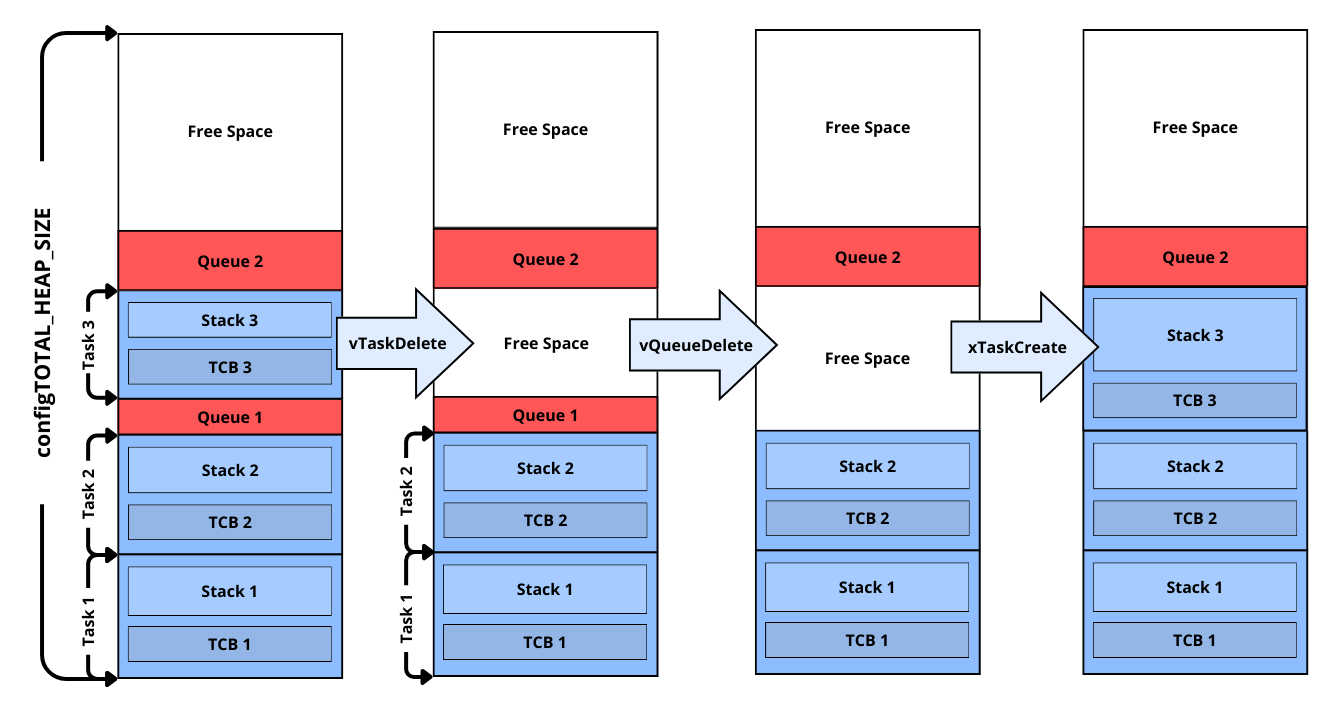
\includegraphics[width=1\linewidth]{resources/images/heap_4.png}
\end{figure}
\end{column}
\end{columns}
\end{frame}

\section{Scheduler}
\begin{frame}{Introducción a FreeRTOS}{Scheduling en FreeRTOS}
\begin{itemize}
    \item El scheduler corre la tarea de mas alta prioridad en estado ready.
    \item Si nada la bloquea, una tarea corre por un tick del RTOS.
    \item Las interrupciones por hardware superan en prioridad a las tareas.
    \item Tareas de misma prioridad en estado ready se alternan.
    \item Si no hay tareas que correr, siempre está la Idle.
\end{itemize}
\begin{figure}
\centering
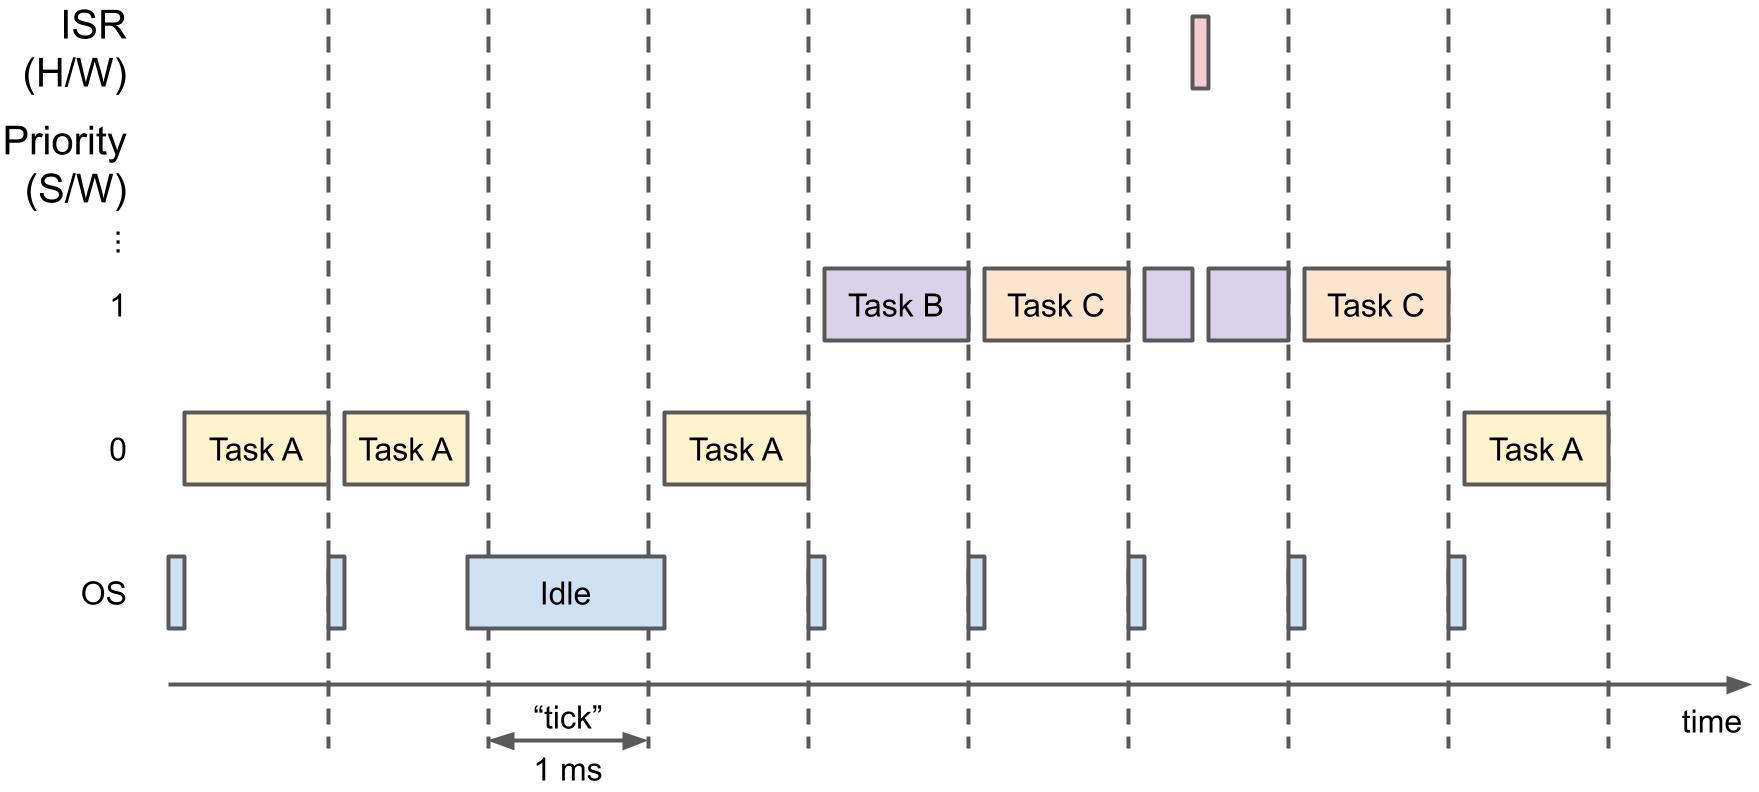
\includegraphics[width=0.5\linewidth]{resources/images/scheduling.png}
\end{figure}
\end{frame}

\section{Tareas}
\subsection{Tareas en FreeRTOS}
\begin{frame}{Introducción a FreeRTOS}{Tareas en FreeRTOS}
\begin{columns}
\begin{column}{0.5\textwidth}
\begin{figure}
\centering
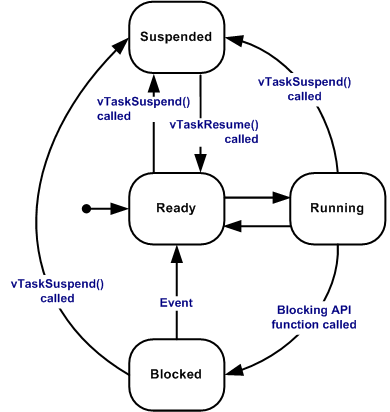
\includegraphics[width=0.8\linewidth]{resources/images/task_states.png}
\end{figure}
\end{column}
\begin{column}{0.5\textwidth}
\begin{itemize}
    \item Son funciones que nunca terminan ni retornan.
    \item Tienen posibles estados de \textit{ready}, \textit{running}, \textit{suspended} y \textit{blocked}.
    \item Tienen stack propio.
    \item Tienen prioridades asociadas.
    \item Se pueden crear y eliminar dinámicamente.
\end{itemize}
\end{column}
\end{columns}
\end{frame}

\subsection{xTaskCreate}
\begin{frame}{Introducción a FreeRTOS}{xTaskCreate - Prototipo}
\begin{columns}
\begin{column}{0.65\textwidth}
La API \textcolor{myblue}{xTaskCreate} se encarga de reservar y registrar los recursos necesarios para correr una tarea.\newline
\begin{enumerate}
    \item \textit{pvTaskCode} es la función que se va a usar de tarea.
    \item \textit{pcName} es el nombre de la tarea en el debugger.
    \item \textit{usStackDepth} es la cantidad de words del stack de la tarea.
    \item \textit{pvParameters} es un puntero a datos que se puedan pasar a la tarea a través de \lstinline[language=c]{void *params}.
    \item \textit{uxPriority} es la prioridad de la tarea.
    \item \textit{pxCreatedTask} es el handle de la tarea.
\end{enumerate}
\end{column}
\begin{column}{0.35\textwidth}
\lstinputlisting[language=c, basicstyle=\tiny]{resources/listings/xTaskCreate.c}
\end{column}
\end{columns}
\end{frame}

\begin{frame}{Introducción a FreeRTOS}{xTaskCreate - Ejemplo}
\begin{columns}
\begin{column}{0.35\textwidth}
\lstinputlisting[language=c, basicstyle=\tiny]{resources/listings/task_create_1.c}
\end{column}
\begin{column}{0.65\textwidth}
\begin{itemize}
    \item \textit{task\_fn} para a ser la función que trabaja de tarea.
    \item En el debugger, vamos a encontrarla con el nombre "Task".
    \item Se asignaron 64 words (256 bytes) de stack.
    \item No se pasan parámetros a la tarea (NULL).
    \item La prioridad es 1 (por encima de IDLE).
    \item No hay handle para la tarea.
\end{itemize}
\end{column}
\end{columns}
\end{frame}

\subsection{Tarea con parámetros}
\begin{frame}{Introducción a FreeRTOS}{xTaskCreate - Parámetros}
\begin{columns}
\begin{column}{0.45\textwidth}
\begin{itemize}
    \item Se pueden pasar parámetros a las tareas casteando el dato como puntero a \textit{void}.
    \item Esto es útil para poder crear varias tareas con la misma función.
    \item El parámetro debe ser casteado al tipo correcto dentro de la tarea.
\end{itemize}
\end{column}
\begin{column}{0.55\textwidth}
\lstinputlisting[language=c, basicstyle=\tiny]{resources/listings/task_params_1.c}
\end{column}
\end{columns}
\end{frame}

\begin{frame}{Introducción a FreeRTOS}{xTaskCreate - Parámetros}
Esta posibilidad hace ofrece una gran ventaja de que se puedan crear tareas más eficientes a partir de una misma función.\newline
\begin{columns}
\begin{column}{0.5\textwidth}
\lstinputlisting[language=c, basicstyle=\tiny]{resources/listings/task_params_2.c}
\end{column}
\begin{column}{0.5\textwidth}
\lstinputlisting[language=c, basicstyle=\tiny]{resources/listings/task_params_3.c}
\end{column}
\end{columns}
\end{frame}

\subsection{Handle de tareas}
\begin{frame}{Introducción a FreeRTOS}{xTaskCreate - Handle}
\begin{columns}
\begin{column}{0.6\textwidth}
\begin{itemize}
    \item Las variables \textcolor{myblue}{TaskHandle\_t} guardan una referencia a una tarea.
    \item Algunas APIs de FreeRTOS usan estas referencias para cambiar propiedades de la tarea. Entre ellas:\newline
    \begin{itemize}
        \item \textcolor{myblue}{vTaskDelete()} que elimina una tarea.
        \item \textcolor{myblue}{uxTaskPriorityGet()} que obtiene la prioridad de una tarea.
        \item \textcolor{myblue}{vTaskPrioritySet()} que setea un nuevo valor de prioridad.
        \item \textcolor{myblue}{vTaskResume()} que reanuda una tarea suspendida.
        \item \textcolor{myblue}{vTaskSuspend()} que suspende una tarea.
    \end{itemize}
\end{itemize}
\end{column}
\begin{column}{0.4\textwidth}
\lstinputlisting[language=c, basicstyle=\tiny]{resources/listings/task_handle.c}
\end{column}
\end{columns}
\end{frame}

\subsection{Bloqueo por tiempo}
\begin{frame}{Introducción a FreeRTOS}{Bloqueo por tiempo}
\begin{columns}
\begin{column}{0.5\textwidth}
Si \textcolor{myblue}{configTICK\_RATE\_HZ} vale 1000, el tick es de 1ms y coinciden los ms con los ticks.
\lstinputlisting[language=c, basicstyle=\tiny]{resources/listings/task_delay_1.c}
Al usar el \textcolor{myblue}{vTaskDelayUntil()} hay que obtener la cantidad de ticks del RTOS. 
\lstinputlisting[language=c,  basicstyle=\tiny]{resources/listings/task_delay_2.c}
Si \textcolor{myblue}{configTICK\_RATE\_HZ} no es 1000, podemos obtener los ticks para una cantidad de ms con una macro:
\lstinputlisting[language=c, basicstyle=\tiny]{resources/listings/task_delay_3.c}
\end{column}
\begin{column}{0.5\textwidth}
\begin{itemize}
    \item \textcolor{myblue}{vTaskDelay()} bloquea la tarea por una determinada cantidad de ticks.
    \item \textcolor{myblue}{vTaskDelayUntil()} bloquea la tarea por una cantidad específica de ticks.
    \item \textcolor{myblue}{vTaskDelay()} bloquea relativo a cuando se llama la API, \textcolor{myblue}{vTaskDelayUntil()} bloquea la tarea por esa cantidad de ticks desde que la tarea se corre.
\end{itemize}
\end{column}
\end{columns}
\end{frame}

\section{Ejercicios}
\begin{frame}{Introducción a FreeRTOS}{Ejercicios}
    Algunas propuestas para practicar
    \noindent\rule{\textwidth}{0.75pt}
    \begin{enumerate}
        \item En un proyecto llamado \textbf{04\_reloj}, hacer un programa que cuente de 00 a 59 en el display 7 segmentos cada 1 segundo. Al llegar a 60 debe volver a empezar en 00.
        \item En un proyecto llamado \textbf{04\_alarma}, armar un sistema de dos tareas donde, al presionar un botón, active una tarea que haga sonar el buzzer. Con otro botón, se activa una tarea que lo apaga.
    \end{enumerate}
    \noindent\rule{\textwidth}{0.75pt}
    Cada ejercicio que se resuelva, subirlo al repositorio personal del curso.
\end{frame}

\section{Referencias}
\begin{frame}{Introducción a FreeRTOS}{Referencias}
    Algunos recursos útiles
    \noindent\rule{\textwidth}{0.75pt}
    \begin{multicols}{2}
    \begin{itemize}
        \item \href{https://github.com/utn-fra-lse/lpc845/blob/main/docs/UM11029.pdf}{Manual del LPC845}
        \item \href{https://github.com/utn-fra-lse/lpc845/blob/main/docs/UM11181.pdf}{Manual del LPC845 Breakout Board}
        \item \href{https://mcuxpresso.nxp.com/api_doc/dev/116/modules.html}{Documentación del SDK del LPC845}
        \item \href{https://github.com/utn-fra-lse/lpc845/blob/main/docs/BASE_KIT_V0.pdf}{Esquemático del kit del laboratorio}
        \item \href{https://www.freertos.org/Documentation/01-FreeRTOS-quick-start/01-Beginners-guide/01-RTOS-fundamentals}{RTOS Fundamentals - FreeRTOS}
        \item \href{https://www.freertos.org/media/2018/FreeRTOS_Reference_Manual_V10.0.0.pdf}{The FreeRTOS Reference Manual}
        \item \href{https://github.com/FreeRTOS/FreeRTOS-Kernel-Book/releases/download/V1.0/Mastering-the-FreeRTOS-Real-Time-Kernel.v1.0.pdf}{Mastering the FreeRTOS Real Time Kernel}
        \item \href{https://www.digikey.ee/en/maker/projects/introduction-to-rtos-solution-to-part-3-task-scheduling/8fbb9e0b0eed4279a2dd698f02ce125f}{RTOS Task Scheduling and Prioritization}
        \item \href{https://www.digikey.com/en/maker/projects/introduction-to-rtos-solution-to-part-4-memory-management/6d4dfcaa1ff84f57a2098da8e6401d9c}{FreeRTOS Memory Management}
    \end{itemize}
    \end{multicols}
\end{frame}

\end{document}
